\documentclass{article}

\usepackage{graphicx}
\usepackage{amsmath}
\usepackage{biblatex}
\usepackage{xcolor}
\usepackage{listings}
\usepackage{xepersian}

\settextfont{Times New Roman}
\addbibresource{references.bib}
\lstdefinestyle{main-style}
{
    backgroundcolor=\color{lightgray},   
	commentstyle=\color{green},
	keywordstyle=\color{teal},
	numberstyle=\tiny\color{gray},
	stringstyle=\color{magenta},
	basicstyle=\ttfamily\footnotesize,
	breakatwhitespace=false,         
	breaklines=true,                 
	captionpos=b,                    
	keepspaces=true,                 
	numbers=left,                    
	numbersep=5pt,                  
	showspaces=false,                
	showstringspaces=false,
	showtabs=false,                  
	tabsize=2
}
\lstset{style=main-style}

\title{میانترم طراحی سیستم‌های دیجیتال}
\author{پارسا محمدیان -- 98102284}

\begin{document}
\maketitle
\newpage
\tableofcontents
\newpage

\section{سوال 3}

\subsection{پیاده سازی پردازنده \lr{subleq}}
برای آشنایی با این معماری از منابع 
\cite{oisc-wikipedia} 
و 
\cite{subleq-esolangs} 
و 
\cite{subleq-game} 
استفاده کردم. 
برای پیاده سازی این پردازنده، ماژول 
\lr{subleq} 
را ساختم و برای سهولت مموری را درون آن به صورت آرایه بیت وکتور در نظر گرفتم که قابلیت لود کردن دارد. 
بقیه جزئیات پیاده‌سازی در کد با کامنت توضیح داده شده است.

\subsection{نوشتن کد مرتب‌سازی}
از آنجایی که 
\lr{Assemble} 
کردن کد این ماشین کار طاقت‌فرسایی است، به زبان پایتون کدی برای اسمبل کردن 
کد این ماشین می‌نویسیم. نمونه کد ورودی 
\lr{Assembler} 
در کد 
\ref{subleq-code}
آمده است. برای راحتی کار کد ورودی را در قالب 
\lr{JSON} 
می‌نویسیم. خروجی این برنامه دستورالعمل‌ها به باینری و آدرس آن‌ها است. اگر پارامتر 
\lr{-d} 
به این برنامه پاس داده شود داده‌ها به همراه آدرسشان در خروجی قرار می‌گیرند. 

\begin{latin}  
\begin{lstlisting}[language=python, caption={Subleq assembler input code}, label={subleq-code}]
{
    "code":[
        {"instruction": "", "op1": "", "op2": "", "jaddr": ""},
        ...
    ],
    "data":[
        "identifer": "value",
        ...
    ]
}
\end{lstlisting}
\end{latin}

برای 
\lr{Assemble} 
کردن کد برنامه را با پارامترهای زیر اجرا می‌کنیم.

\begin{latin}
	\lstinline[language=python]{python assembler.py -d -i "input.json" -o "output.txt"}
\end{latin}

حال کد بابل سورت و دیتا را می‌نویسیم و به کمک این زبان آن را به کد ماشین متناظر تبدیل می‌کنیم. کد این بخش در فایل 
\lr{sort.json} 
موجود است.

\subsection{اجرای کد بر روی پردازنده}
اگر پارامتر 
\lr{-v} 
را به اسمبلر پاس دهیم کد لود کردن در مموری را برای وریلاگ به ما می‌دهد. این کد را در فایل 
\lr{sort.v} 
و در ماژولی با همین نام قرار می‌دهیم. سپس با شبیه سازی نتیجه را بررسی می‌کنیم.

\section{سوال 7}
\subsection{جزئیات پیاده‌سازی}
برای آشنایی با  
\lr{TCAM} 
از منابع 
\cite{tcam-searchnetworking}
و
\cite{tcam-wikipedia}
استفاده کردم. همچنین از تمرین پنجم درس ساختار و زبان کامپیوتر پائیز 1399 دکتر ارشدی که در مورد 
\lr{CAM} 
بود نیز استفاده کردم. سپس برای پیاده‌سازی از توصیف رفتاری استفاده کردم. در کد از دو پارامتر 
\lr{N}
و 
\lr{WORD\_SIZE} 
استفاده شده است که 
\lr{N} 
طول آدرس است. نکته قابل توجه این است که علی رغم اینکه وریلاگ در منطق خود 
\lr{X} 
دارد ولی در سنتز چنین چیزی وجود ندارد چون یک سیم حتی اگر مقدارش را ندانیم دارای مقدار است. 
پس باید خودمان منطق سه تایی را پیاده سازی کنیم. برای این کار برای هر داده علاوه بر خود داده، 
وکتور دیگری در نظر گرفته شده که 1 بودن هر خانه از آن مشخص کننده 
\lr{X} 
بودن خانه متناظر در داده است. با این تفاصیل سراغ پیاده سازی می‌رویم. پیاده سازی در فایل 
\lr{tcam.v} 
موجود است.

\subsection{جزئیات تست}
برای تست فایل 
\lr{tcam\_tb.v} 
نوشته شده است. در این تست ابتدا مقادیری در حافظه ذخیره شده که همه بیت های آن ها مشخص است. 
سپس هر یک از مقادیر فراخوانی شده است و آدرس متناظر دریافت شده است. پس از این ها به سراغ تست نوشتن با 
\lr{X} 
میرویم. سپس با دو مقدار متفاوت که در بیت نامعلومشان اختلاف دارند آدرس را می‌گیریم. 
\lr{Wave} 
مربوط به این تست در شکل 
\ref{tcam-wave}
نشان داده شده است.

\begin{figure}[!htbp]
	\centering
	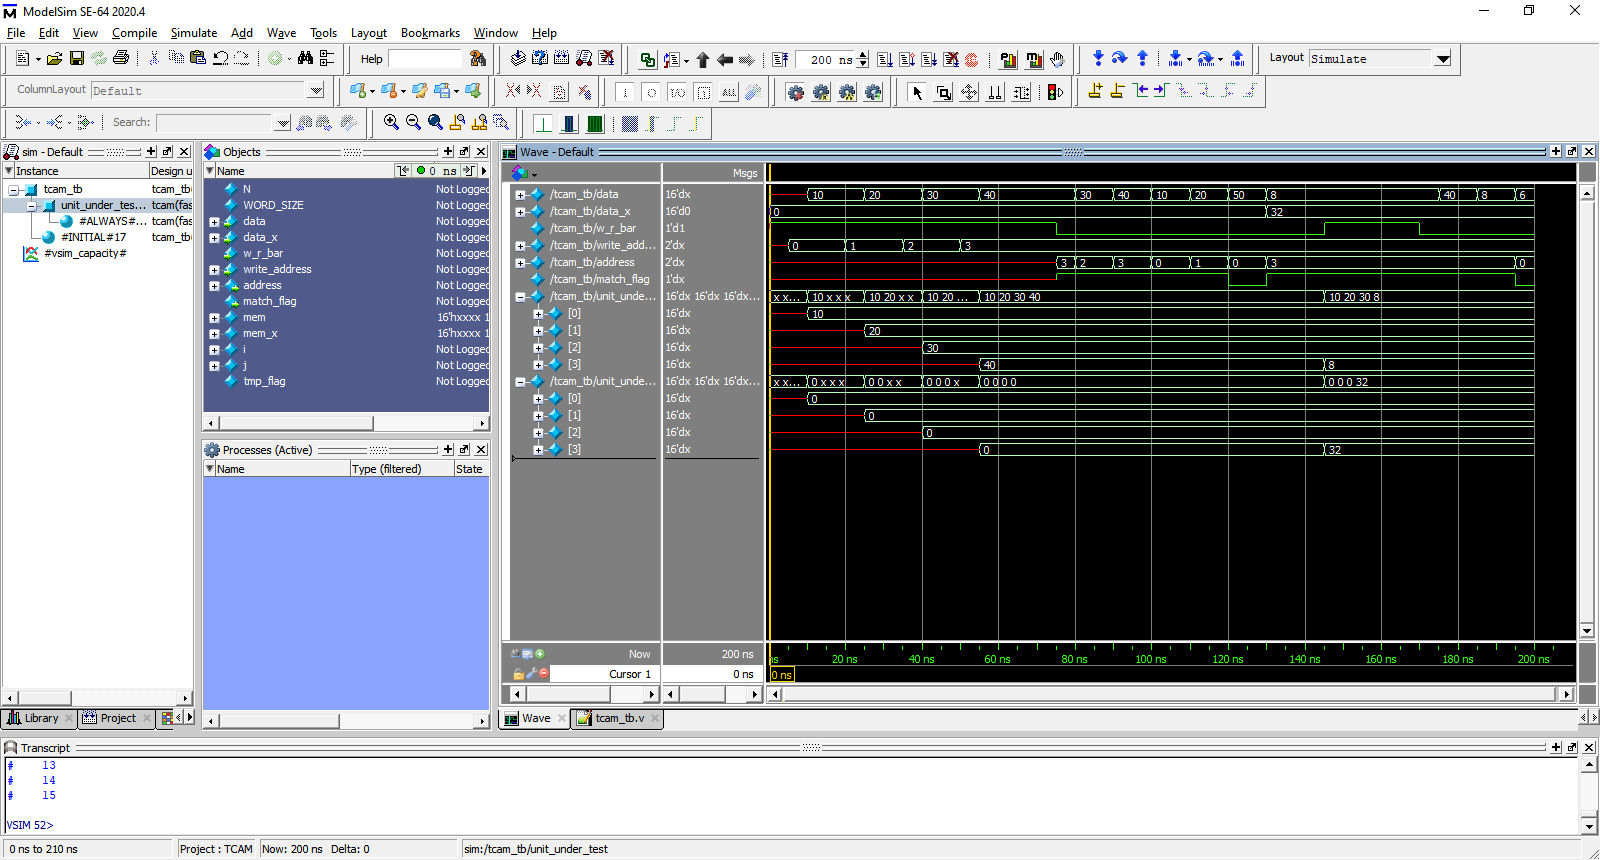
\includegraphics[width=\linewidth]{tcam_tb_wave.png}
	\caption{شکل موج تست \lr{TCAM}}
	\label{tcam-wave}
\end{figure}


\section{سوال 9}
برای حل این سوال ابتدا با 
\lr{Array Multiplier} 
از طریق 
\cite{array-multiplier-elprocus} 
و 
\cite{array-multiplier-youtube} 
آشنا شدم. سپس برای پیاده سازی از شکل 
\ref{elprocus-pic}
که در منبع اول موجود بود استفاده کردم. 
\begin{figure}[!htbp]
	\centering
	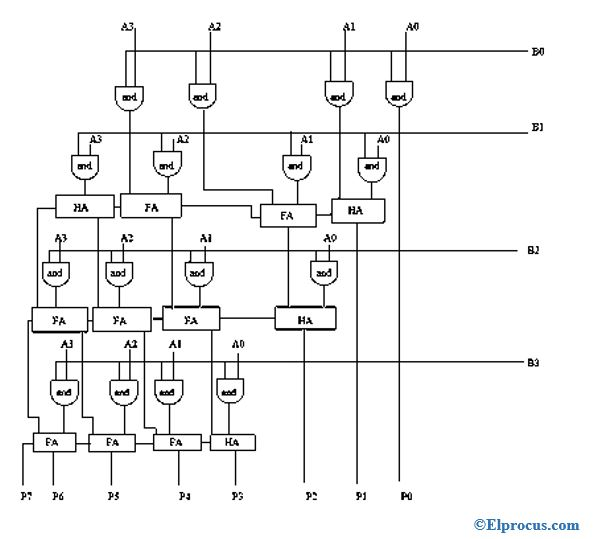
\includegraphics[width=\linewidth]{logic-diagram-of-4-by-4-array-multiplier.jpg}
	\caption{\lr{Array Multiplier}}
	\label{elprocus-pic}
\end{figure}
لازم به ذکر است که برای سادگی در کد، ماژول 
\lr{part} 
را به صورت ترکیب 
\lr{fa} 
و گیت 
\lr{and} 
تعریف کردم. در این صورت به ازای هر بخش از این ماتریکس از این 
ماژول استفاده کردم. برای مثال اگر فقط نیاز به گیت 
\lr{and} 
دو ورودی دیگر را صفر می‌دهیم. جزئیات دیگر کد پایتون تقریبا واضح است. 
برای تست یکی ضرب‌کننده 4 در 4 می‌سازیم و برای آن تست بنچ می‌نویسیم. تست بنچ در ماژول 
\lr{stimulus} 
است.

\newpage
\section*{فهرست منابع}
\begin{latin}
    \printbibliography[heading=bibintoc, title=فهرست منابع]
\end{latin}

\end{document}